\providecommand{\main}{../../..}
\documentclass[\main/main.tex]{subfiles}
\begin{document}

\subsection{Esercizio 4}
Si determini la soluzione preferita assegnando al primo indicatore peso pari alla metà del secondo $(\w_1 = \w2_/2)$.

\begin{align*}
  \max f_1 = -x_1 -x_2  \\
  \max f_2 = x_1        \\
  3x_1^2 + 4x_2 \leq 12 \\
  x_2 \geq 0
\end{align*}

\subsection{Risoluzione esercizio 4}

\subsubsection*{Costruisco funzione obbiettivo}
\[
  f^* = \frac{1}{2}x_1 - x_2
\]

\subsubsection*{Risolvo il problema}

\begin{align*}
  \max f^* = \frac{1}{2}x_1 - x_2 \\
  3x_1^2 + 4x_2 \leq 12
  x_2 \geq 0
\end{align*}

Il valore minimo di $x_2$ è $0$, mentre il valore massimo di $x_1 = 2$.

\subsubsection*{Verifico la soluzione}

\begin{figure}
  \begin{subfigure}{0.45\textwidth}
    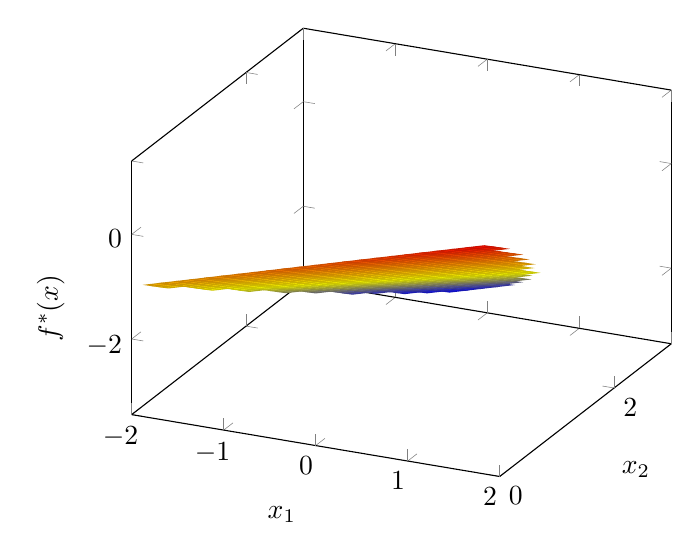
\begin{tikzpicture}
      \begin{axis}[
          xlabel=$x_1$,
          ylabel=$x_2$,
          zlabel=$f^*(x)$,
          domain=-2:2,
          y domain=0:3
        ]
        \addplot3[surf, unbounded coords=jump]
        {3*x^2 + 4*y <= 12 ? 0.5*x-y : NaN};
      \end{axis}
    \end{tikzpicture}
    \caption{La funzione $f^*(x)$}
  \end{subfigure}
  ~
  \begin{subfigure}{0.45\textwidth}
    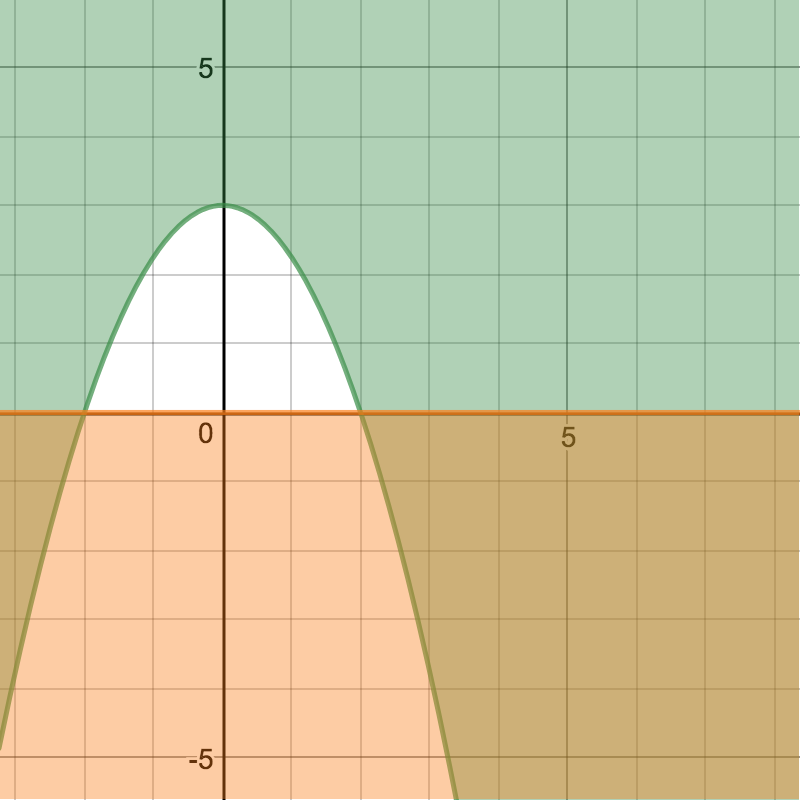
\includegraphics[width=0.8\textwidth]{es4-maut}
    \caption{Dominio della funzione $f^*(x)$}
  \end{subfigure}
\end{figure}

\end{document}